% !TEX root = ./article.tex

\documentclass{article}

\usepackage{mystyle}
\usepackage{myvars}

%-----------------------------

\begin{document}

	\maketitle
  \thispagestyle{empty}

%-----------------------------
%	TEXT
%-----------------------------


	\section{Sea $X$ una v. a. normal con media $\mu = 0$ y varianza $\sigma^2 = 1$, es decir, $ X \sim N(0,1)$. Hallar la función de densidad de la v.a. $Y = X^2$}

    \paragraph{}
    Para obtener la función de densidad de la variable transformada se seguirá la ecuación \eqref{eq:density_transformation_technique}. Esta se cumple cuando la función $f_X$ es monotona creciente. Sin embargo, en este caso se deberá adaptar a trozos para que esta sea así, puesto que la función de densidad de la variable normal tiene forma de montículo (\say{\emph{Campana de Gauss}}).


    \begin{equation}
      f_X(x) = {\displaystyle {\frac {1}{\sqrt {2\pi \sigma ^{2}}}}\,e^{-{\frac {(x-\mu )^{2}}{2\sigma ^{2}}}}} \implies f_X(x) = \frac{1}{\sqrt{2\pi} } e^{-\frac{x^2}{2}}, \ x \in \mathbb{R}
    \end{equation}


    \begin{align}
      g(x) =& x^2 \\
      g^{-1}(x) =& \pm \sqrt{x} \\
      \left| \frac{d}{dx} g^{-1} (x) \right| =& \left| \pm \frac{1}{2\sqrt{x}}  \right| = \frac{1}{2\sqrt{x}}
    \end{align}

    \begin{equation}
    \label{eq:density_transformation_technique}
      f_Y (y) = \sum f_X \left( g^{-1} (y) \right) \left| \frac{d}{dy} g^{-1} (y) \right|
    \end{equation}

    \begin{align}
      f_Y (y) =& &\\
              =& \sum f_X \left( g^{-1} (y) \right) \left| \frac{d}{dy} g^{-1} (y) \right| &\\
              =& f_X \left( \sqrt{y} \right) \left| \frac{d}{dy} g^{-1} (y) \right| + f_X \left( - \sqrt{y} \right) \left| \frac{d}{dy} g^{-1} (y) \right| &\\
              =& 2f_X \left( \sqrt{y} \right) \left| \frac{d}{dy} g^{-1} (y) \right| &\\
              =& 2f_X \left( \sqrt{y} \right) \left| \pm \frac{1}{2\sqrt{y}} \right| &\\
              =& 2f_X \left( \sqrt{y} \right) \frac{1}{2\sqrt{y}} &\\
              =& 2\frac{1}{\sqrt{2\pi} } e^{-\frac{y}{2}} \frac{1}{2\sqrt{y}}  & \\
              =& \frac{e^{-\frac{y}{2}}}{ \sqrt{2\pi} \sqrt{y} } & 0<y<\infty
    \end{align}

    \begin{figure}
      \center
      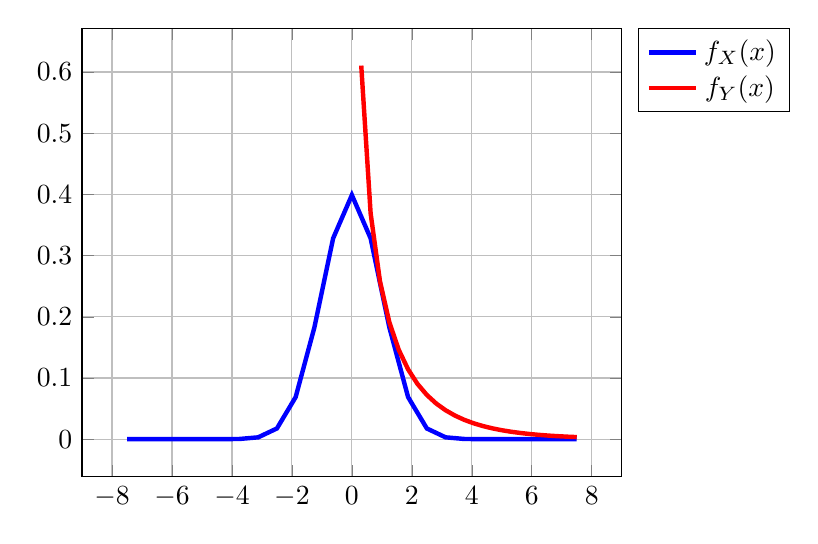
\begin{tikzpicture}
          \begin{axis}[
            legend pos=outer north east,
            grid=both,
            xtick distance=2,
            ytick distance=0.1,
            every axis plot/.append style={ultra thick}
          ]
            \addplot[color=blue][domain=-7.5:7.5]{e^(- (x^2 / 2))/(sqrt(2 * pi))};
            \addplot[color=red][domain=0:7.5] {e^(-x / 2)/(sqrt(2 * pi)*sqrt(x))};
          \legend{ $f_X(x)$, $f_Y(x)$}
          \end{axis}
      \end{tikzpicture}
      \caption{}
      \label{}
    \end{figure}

    \paragraph{}
    Debido a

  \section{Sea $X$ una v. a. uniformemente distribuida en $[0,2\pi]$, es decir, con función de densidad $f(x)=\frac{1}{2\pi}, \ x \in (0,2\pi)$. Hallar la función de densidad de la v.a. $Y = \cos(X)$}

    \paragraph{}
    [TODO]


    \begin{equation}
      f_X(x) = \frac{1}{2\pi}, \ 0 < x < 2\pi
    \end{equation}


    \begin{align}
      g(x) =& \cos(x) \\
      g^{-1}(x) =& \arccos(x) \\
      \left| \frac{d}{dx} g^{-1} (x) \right| =& \left| - \frac{1}{\sqrt{1-x^2}} \right| =  \frac{1}{\sqrt{1-x^2}}
    \end{align}

    \begin{equation}
    \label{eq:density_transformation_technique}
      f_Y (y) = \sum f_X \left( g^{-1} (y) \right) \left| \frac{d}{dy} g^{-1} (y) \right|
    \end{equation}

    \begin{figure}
      \center
      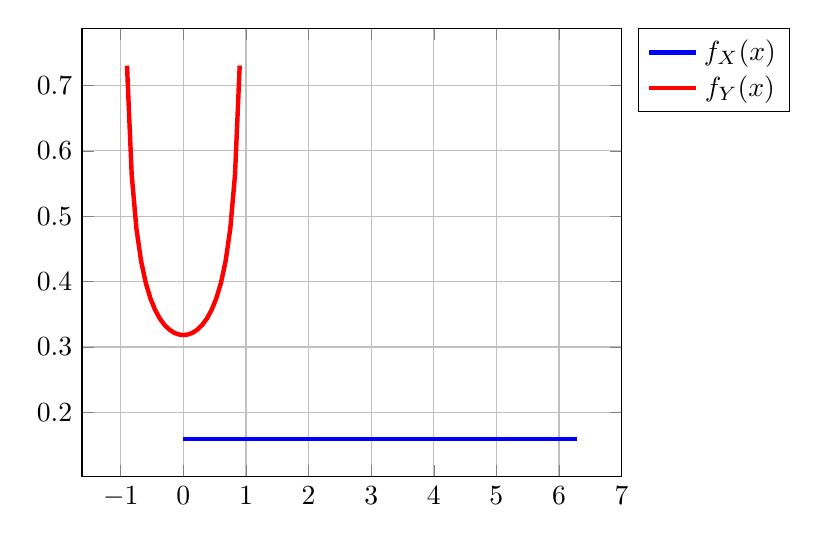
\begin{tikzpicture}
          \begin{axis}[
            legend pos=outer north east,
            grid=both,
            xtick distance=1,
            ytick distance=0.1,
            every axis plot/.append style={ultra thick}
          ]
            \addplot[color=blue][domain=0:2*pi]{1/(2*pi)};
            \addplot[color=red][domain=-0.9:0.9] {1 / (pi * sqrt(1-x^2))};
          \legend{ $f_X(x)$, $f_Y(x)$}
          \end{axis}
      \end{tikzpicture}
      \caption{}
      \label{}
    \end{figure}

    \begin{align}
      f_Y (y) =& &\\
              =& \sum f_X \left( g^{-1} (y) \right) \left| \frac{d}{dy} g^{-1} (y) \right| &\\
              =& 2\frac{1}{2\pi} \left| \frac{d}{dy} g^{-1} (y) \right| &\\
              =& 2\frac{1}{2\pi}*\frac{1}{\sqrt{1-y^2}} &\\
              =& \frac{1}{\pi\sqrt{1-y^2}} & -1<y<1
    \end{align}
%-----------------------------
%	Bibliographic references
%-----------------------------
  \nocite{prob2017}

  \bibliographystyle{alpha}
  \bibliography{bib}

\end{document}
